%%%%%%%%%%%%%%%%%%%%%%%%%%%%%%%%%%%%%%%%%%%%%%%%%%%
%% LaTeX book template                           %%
%% Author:  Amber Jain (http://amberj.devio.us/) %%
%% License: ISC license                          %%
%%%%%%%%%%%%%%%%%%%%%%%%%%%%%%%%%%%%%%%%%%%%%%%%%%%

\documentclass[a4paper,11pt,oneside]{book}

\usepackage[T1]{fontenc}
\usepackage[utf8]{inputenc}
\usepackage{lmodern}
\usepackage{csquotes}
\usepackage{amsmath}
\usepackage{nicefrac}
\usepackage{breqn}
\usepackage{pgfplots}
\usepackage{tikz}


\usepackage{titletoc}%

  \titlecontents{chapter}[0em]{\lsstyle\smallskip\bfseries}%\vspace{1cm}%
  {}%
  {\itshape\bfseries}%numberless%
  {\hfill\contentspage}[\medskip]%
%
 \titlecontents{section}[4.25em]{\smallskip}%
  {\contentslabel[\thecontentslabel]{2em}}%numbered
  {\hspace*{-1em}}%numberless
  {\hfill\contentspage}[\smallskip]%
%
 \titlecontents{subsection}[7em]{}%
  {\contentslabel[\thecontentslabel]{2.75em}}%numbered
  {\hspace*{-1em}}%numberless
  {\hfill\contentspage}[\smallskip]


\setcounter{secnumdepth}{0}

\usepackage[margin=1.25in]{geometry}

%%%%%%%%%%%%%%%%%%%%%%%%%%%%%%%%%%%%%%%%%%%%%%%%%%%%%%%%%
% Source: http://en.wikibooks.org/wiki/LaTeX/Hyperlinks %
%%%%%%%%%%%%%%%%%%%%%%%%%%%%%%%%%%%%%%%%%%%%%%%%%%%%%%%%%
\usepackage{hyperref}
\usepackage{graphicx}
\usepackage[english]{babel}

%%%%%%%%%%%%%%%%%%%%%%%%%%%%%%%%%%%%%%%%%%%%%%%%%%%%%%%%%%%%%%%%%%%%%%%%%%%%%%%%
% 'dedication' environment: To add a dedication paragraph at the start of book %
% Source: http://www.tug.org/pipermail/texhax/2010-June/015184.html            %
%%%%%%%%%%%%%%%%%%%%%%%%%%%%%%%%%%%%%%%%%%%%%%%%%%%%%%%%%%%%%%%%%%%%%%%%%%%%%%%%
\newenvironment{dedication}
{
\cleardoublepage%
\thispagestyle{empty}
\vspace*{\stretch{1}}
\hfill\begin{minipage}[t]{0.66\textwidth}
\raggedright%
}
{
   \end{minipage}
   \vspace*{\stretch{3}}
   \clearpage
}

%%%%%%%%%%%%%%%%%%%%%%%%%%%%%%%%%%%%%%%%%%%%%%%%
% Chapter quote at the start of chapter        %
% Source: http://tex.stackexchange.com/a/53380 %
%%%%%%%%%%%%%%%%%%%%%%%%%%%%%%%%%%%%%%%%%%%%%%%%
\makeatletter
\renewcommand{\@chapapp}{}% Not necessary...
\newenvironment{chapquote}[2][2em]
  {\setlength{\@tempdima}{#1}%
   \def\chapquote@author{#2}%
   \parshape 1 \@tempdima \dimexpr\textwidth-2\@tempdima\relax%
   \itshape}
  {\par\normalfont\hfill--\ \chapquote@author\hspace*{\@tempdima}\par\bigskip}
\makeatother

\newcommand{\pder}[2]{\frac{\partial #1}{\partial #2}}
\newcommand{\der}[2]{\frac{\mathrm{d} #1}{\mathrm{d} #2}}
\newcommand{\peren}[1]{\left( #1 \right)}
\newcommand{\brac}[1]{\left[] #1 \right]}




%%%%%%%%%%%%%%%%%%%%%%%%%%%%%%%%%%%%%%%%%%%%%%%%%%%
% First page of book which contains 'stuff' like: %
%  - Book title, subtitle                         %
%  - Book author name                             %
%%%%%%%%%%%%%%%%%%%%%%%%%%%%%%%%%%%%%%%%%%%%%%%%%%%

% Book's title and subtitle
\title{\Huge \textbf{18.02: Multivariable Calculus} \\ \huge Problem Set 4 \\ \large As taught by \textsc{Prof.\ John Bush}, MIT}
% Author
\author{\textsc{Jackson Kearl}}


\begin{document}

\maketitle

%%%%%%%%%%%%%%%%%%%%%%%%%%%%%%%%%%%%%%%%%%%%%%%%%%%%%%%%%%%%%%%%%%%%%%%%
% Auto-generated table of contents, list of figures and list of tables %
%%%%%%%%%%%%%%%%%%%%%%%%%%%%%%%%%%%%%%%%%%%%%%%%%%%%%%%%%%%%%%%%%%%%%%%%
\let\cleardoublepage\clearpage
\tableofcontents
\let\cleardoublepage\clearpage
\mainmatter%

%%%%%%%%%%%
% Preface %
%%%%%%%%%%%
\chapter*{Introduction}

\begin{chapquote}{Lewis Carroll, \textit{Alice in Wonderland}}
``Begin at the beginning,'' the King said, gravely, ``and go on till you
come to an end; then stop.''
\end{chapquote}

\section*{Course Content}
This course covers aspects of calculus involving:
\begin{displayquote}
Calculus of several variables. Vector algebra in 3-space, determinants, matrices.
 Vector-valued functions of one variable, space motion. Scalar functions of several variables: partial differentiation, gradient, optimization techniques.  Double integrals and line integrals in the plane; exact differentials and  conservative fields; Green's theorem and applications, triple integrals, line and surface integrals in space, Divergence theorem, Stokes' theorem;  applications.\footnote{\url{http://student.mit.edu/catalog/m18a.html##18.02}}
\end{displayquote}


\section*{Structure of Homework}
% You might want to add short description about each chapter in this book.
Problems will be arranged as they are on the assigment page. Problems broken into parts one and two, as per assignment page. Within part one, problems divided first by Lecture number, then by book section.

\section*{Distribution}
All relevant notes and information are made available on github\footnote{\url{https://github.com/JacksonKearl/MIT}}.
This includes:
\begin{itemize}
  \item Plaintext notes from lecture and recitation
  \item The raw .tex and .md source for these PDF's
  \item These PDF files
\end{itemize}

\noindent Licensed under Creative Commons Attribution-ShareAlike 4.0 International License.\footnote{\url{http://creativecommons.org/licenses/by-sa/4.0/}}
\let\cleardoublepage\clearpage


%%%%%%%%%%%%%%%%
% NEW CHAPTER! %
%%%%%%%%%%%%%%%%
\begingroup
\let\cleardoublepage\clearpage
\part{Book}
\endgroup


\chapter{Lecture 12}

\section{Section 13.9}

\subsection{Problem 2}\label{problem-2}

\begin{enumerate}
\item
  Define Functions:

  \begin{align*}
  \text{Function: }& &f(x,y) &= x + y \\
  \text{Constraint: }& &x^2 + 4y^2 &= 1
  \end{align*}


\item
  Rearrange such that the condition is satisfied when \(g(x,y) = 0\):
  \[g(x,y) = x^2 + 4y^2 - 1\]
\item
  Plug into Lagrange Multiplier equation,
  \(L(x,y,\lambda) = f(x,y)-\lambda g(x,y)\):
  \[L(x, y, \lambda) = x + y - \lambda(x^2 + 4y^2 - 1)\]
\item
  Take partials with respect to \(x\), \(y\), and \(\lambda \), and set
  to \(0\):
  \[\frac{\partial L}{\partial x} = 1 - 2\lambda x = 0 \Longrightarrow x = \frac{1}{2\lambda}\]
  \[\frac{\partial L}{\partial y} = 1 - 8\lambda y = 0 \Longrightarrow y = \frac{1}{8\lambda}\]
  \[\frac{\partial L}{\partial \lambda} = x^2 + 4y^2 - 1 = 0\]
\item
  Solve as a system of equations:

  \begin{align*}
  \frac{1}{2\lambda}^2 + 4 \frac{1}{8\lambda}^2 -1 &= 0 \\
  \frac{1}{4\lambda^2} + 4 \frac{1}{64\lambda^2} -1 &= 0 \\
  \frac{4}{16\lambda^2} + \frac{1}{16\lambda^2} -1 &= 0 \\
  \frac{5}{16\lambda^2} &= 1 \\
  \lambda &= \pm \frac{\sqrt{5}}{4}
  \end{align*}


\item
  Substitute back to find \(x\) and \(y\):\\


  \begin{align*}
  x = \frac{\pm4}{2\sqrt{5}} &= \frac{\pm2}{\sqrt{5}}\\
  y = \frac{\pm4}{8\sqrt{5}} &= \frac{\pm1}{2\sqrt{5}}
  \end{align*}


\item
  Empirically determine minimum and maximum from original \(f(x,y)\):


  \begin{align*}
  \text{Minimum: }& &f \left(\frac{-2}{\sqrt{5}}, \frac{-1}{2\sqrt{5}}\right) = \frac{-2}{\sqrt{5}} + \frac{-1}{2\sqrt{5}} &= \frac{-5}{2\sqrt{5}}\\
  \text{Maximum: }& &f \left(\frac{2}{\sqrt{5}}, \frac{1}{2\sqrt{5}}\right) = \frac{2}{\sqrt{5}} +\frac{1}{2\sqrt{5}} &= \frac{5}{2\sqrt{5}}
  \end{align*}


\end{enumerate}

\subsection{Problem 8}\label{problem-8}

\begin{enumerate}

\item
  Define Functions:

  \begin{align*}
  \text{Function: }& &f(x,y,z) &= 3x + 2y + z\\
  \text{Constraint: }& &x^2 + y^2 + z^2 &= 1
  \end{align*}


\item
  Rearrange such that the condition is satisfied when \(g(x,y,z) = 0\):
  \[g(x,y) = x^2 + y^2 + z^2 - 1\]
\item
  Plug into Lagrange Multiplier equation,
  \(L(x,y,z,\lambda) = f(x,y,z)-\lambda g(x,y,z)\)
  \[L(x, y, z, \lambda) = 3x + 2y + z - \lambda(x^2 + y^2 + z^2 - 1)\]
\item
  Take partials with respect to \(x\), \(y\), \(z\), and \(\lambda \),
  and set to \(0\):
  \[\frac{\partial L}{\partial x} = 3 - 2\lambda x = 0 \Longrightarrow x = \frac{3}{2\lambda}\]
  \[\frac{\partial L}{\partial y} = 2 - 2\lambda y = 0 \Longrightarrow y = \frac{1}{\lambda}\]
  \[\frac{\partial L}{\partial z} = 1 - 2\lambda z = 0 \Longrightarrow z = \frac{1}{2\lambda}\]
  \[\frac{\partial L}{\partial \lambda} = x^2 + y^2 + z^2 - 1 = 0\]
\item
  Solve as a system of equations:

  \begin{align*}
  \frac{3}{2\lambda}^2 + \frac{1}{\lambda}^2 + \frac{1}{2\lambda}^2-1 &= 0 \\
  \frac{9}{4\lambda^2} + \frac{1}{\lambda^2} + \frac{1}{4\lambda^2} -1 &= 0 \\
  \frac{9}{4\lambda^2} + \frac{4}{4\lambda^2} + \frac{1}{4\lambda^2} -1 &= 0 \\
  \frac{14}{4\lambda^2} -1 &= 0 \\
  \frac{7}{2\lambda^2} &= 1 \\
  \lambda &= \pm \frac{\sqrt{14}}{2}
  \end{align*}


\item
  Substitute back to find \(x\) and \(y\):

  \begin{align*}
  x &= \pm\frac{3}{\sqrt{14}}\\
  y &= \pm\frac{2}{\sqrt{14}}\\
  z &= \pm\frac{1}{\sqrt{14}}
  \end{align*}


\item
  Empirically determine min and max from original \(f(x,y)\):

  \begin{align*}
  \text{Min: }& &f \left(\frac{-3}{\sqrt{14}}, \frac{-2}{\sqrt{14}}, \frac{-1}{\sqrt{14}}\right) =3\frac{-3}{\sqrt{14}}+ 2\frac{-2}{\sqrt{14}}+ \frac{-1}{\sqrt{14}} = \frac{-14}{\sqrt{14}}\\
  \text{Max: }& &f \left(\frac{3}{\sqrt{14}}, \frac{2}{\sqrt{14}}, \frac{1}{\sqrt{14}}\right) =3\frac{3}{\sqrt{14}}+ 2\frac{2}{\sqrt{14}}+ \frac{1}{\sqrt{14}} = \frac{14}{\sqrt{14}}
  \end{align*}


\end{enumerate}

\subsection{Problem 38}\label{problem-38}

\begin{enumerate}

\item
  Define Functions:

  \begin{align*}
  \text{Function: }& &f(x,y) &= x^2 + y^2\\
  \text{Constraint: }& &x^2 + xy + y^2 &= 3
  \end{align*}


\item
  Rearrange such that the condition is satisfied when \(g(x,y) = 0\):
  \[g(x,y) = x^2 + xy + y^2 - 3\]
\item
  Plug into Lagrange Multiplier equation,
  \(L(x,y,\lambda) = f(x,y)-\lambda g(x,y)\)
  \[L(x, y, \lambda) = x^2 + y^2 - \lambda(x^2 + xy + y^2 - 3)\]
\item
  Take partials with respect to \(x\), \(y\), and \(\lambda \), and set
  to \(0\):
  \[\frac{\partial L}{\partial x} = 2x - 2\lambda x - \lambda y= 0 \Longrightarrow x = \frac{\lambda y}{2 - 2\lambda}\]
  \[\frac{\partial L}{\partial y} = 2y - 2\lambda y - \lambda x= 0 \Longrightarrow y = \frac{\lambda x}{2 - 2\lambda}\]
  \[\frac{\partial L}{\partial \lambda} = x^2 + xy + y^2 - 3 = 0\]
\item
  Solve as a system of equations:

  \begin{align*}
  x &= \frac{\lambda y}{2-2\lambda}& && y &= \frac{\lambda x}{2-2\lambda}\\
  \frac{x}{y} &= \frac{\lambda}{2-2\lambda}& && \frac{y}{x} &= \frac{\lambda}{2-2\lambda}\\
  &&\frac{x}{y} &= \frac{y}{x}\\
  &&x^2 &= y^2\\
  &&y &= \pm x\\
  g(x,y) = 3x^2 - 3 &= 0 &&& g(x,y) =x^2-3 &= 0\\
  3x^2 &= 3 &&& x^2 &= 3\\
  x^2 &= 1 &&& x^2 &= 3\\
  x =y &= \pm1 &&& x =-y&= \pm\sqrt{3}\\
  \end{align*}


\item
  Substitute back to find \(x\) and \(y\):

  \begin{align*}
  (x,y) = (1,1),\space(-1,-1),\space(\sqrt{3},-\sqrt{3}),\space(-\sqrt{3},\sqrt{3})
  \end{align*}


\item
  Empirically determine min and max from original \(f(x,y)\):

  \begin{align*}
  \text{Distance from Origin:} &&D(x,y) &= \sqrt{x^2 + y^2}\\
  \text{Minimums @ }(1,1),\space(-1,-1): & &D(1,1) =  D(-1,-1)&= \sqrt{2}\\
  \text{Maximums @ }(-\sqrt{3},\sqrt{3}),\space(\sqrt{3},-\sqrt{3}): & &D(-\sqrt{3},\sqrt{3})&= \sqrt{6}
  \end{align*}


\end{enumerate}

\subsection{Problem 52}\label{problem-52}

\begin{enumerate}
\def\labelenumi{\arabic{enumi}.}
\item
  Define Functions:

  \begin{align*}
  \text{Function: }& &f(x,y) &= (x-3)^2 + (y-2)^2\\
  \text{Constraint: }& &4x^2 + 9y^2 &= 36
  \end{align*}


\item
  Rearrange such that the condition is satisfied when \(g(x,y) = 0\):
  \[g(x,y) = 4x^2 + 9y^2 -36\]
\item
  Plug into Lagrange Multiplier equation,
  \(L(x,y,\lambda) = f(x,y)-\lambda g(x,y)\)
  \[L(x, y, \lambda) = (x-3)^2 + (y-2)^2 - \lambda(4x^2 + 9y^2 - 36)\]
\item
  Take partials with respect to \(x\), \(y\), and \(\lambda \), and set
  to \(0\):
  \[\frac{\partial L}{\partial x} = 2x - 6 -8\lambda x= 0 \Longrightarrow x = \frac{3}{1 - 4\lambda}\]
  \[\frac{\partial L}{\partial y} = 2y - 4-18\lambda y= 0 \Longrightarrow y = \frac{2}{1 - 9\lambda}\]
  \[\frac{\partial L}{\partial \lambda} = 4x^2 + 9y^2 - 36 = 0\]
\item
  Solve as a system of equations, using CAS software:

  \begin{align*}
  4x^2 + 9y^2 - 36 &= 0\\
  4\left(\frac{3}{1 - 4\lambda}\right)^2 + 9\left(\frac{2}{1 - 9\lambda}\right)^2 - 36 &= 0\\
  \lambda &= [0.5103, -0.0684]
  \end{align*}


\item
  Substitute back to find \(x\) and \(y\):

  \[(x,y) = \left(\frac{3}{1 - 4\lambda},\frac{2}{1 - 9\lambda}\right)\]

  \begin{align*}
  (x,y) &= \left(\frac{3}{1 - 4(0.5103)},\frac{2}{1 - 9(0.5103)}\right) & \text{OR  } & (x,y) = \left(\frac{3}{1 - 4(-0.0684)},\frac{2}{1 - 9(-0.0684)}\right)\\
  (x,y) &= \left(-2.88, -0.557\right) & \text{OR  } & (x,y) = (2.36,1.24)
  \end{align*}


\item
  Empirically determine min and max from original \(f(x,y)\):

  \begin{align*}
  \text{Distance from Origin:} &&D(x,y) = \sqrt{(x-3)^2 + (y-2)^2}\\
  \text{Minimum @ }(2.36,1.24): & &D(2.36,1.24) = 0.993\\
  \text{Maximum @ }(-2.88, -0.557): & &D(-2.88, -0.557)= 6.411
  \end{align*}


\end{enumerate}

\section{Section 13.10}\label{section-13.10}

\subsection{Problem 4}\label{problem-4}

\begin{enumerate}

\item
  Calculate partials, set to 0 to find critical points:

  \begin{align*}
  \frac{\partial f}{\partial x} = y+3= 0 &\Longrightarrow y = -3\\
  \frac{\partial f}{\partial y} = x - 2= 0 &\Longrightarrow x = 2
  \end{align*}


\item
  Evaluate discriminant at critical point, \((2,-3)\):

  \begin{align*}
  \Delta &= f_{xx}(x,y)\space f_{yy}(x,y) - [f_{xy}(x,y)]^2\\
  &= 0\cdot0-1\\
  &= -1
  \end{align*}

   The discriminant at \((2,-3)\) is negative, meaning there is a
  saddle point here, not a minimum or maximum.
\end{enumerate}

\subsection{Problem 10}\label{problem-10}

\begin{enumerate}

\item
  Calculate partials, set to 0 to find critical points:

  \begin{align*}
  \frac{\partial f}{\partial x} = 3y - 3x^2 &= 0 &\Longrightarrow y = x^2\\
  \frac{\partial f}{\partial y} = 3x - 3y^2 &= 0 &\Longrightarrow x = y^2\\
  x &= x^4 &\Longrightarrow (x,y) = (0,0)\\
  1 &= x^3 &\Longrightarrow (x,y) = (1,1)\\
  \end{align*}


\item
  Evaluate discriminant at critical points \((0,0)\), and \((1,1)\):

  \begin{align*}
  \Delta(x,y) &= f_{xx}(x,y)\space f_{yy}(x,y) - [f_{xy}(x,y)]^2\\
  &= -6x \cdot -6y - [3]^2\\
  \Delta(0,0)&=0 \cdot 0 - 9 = -9\\
  \Delta(1,1)&= -6 \cdot -6 - 9 = 27
  \end{align*}

   The discriminant at \((0,0)\) is negative, meaning it is a saddle
  point, not a minima or maxima.

  However, the discriminant at \((1,1)\) is positive, meaning it is
  either a minima or maxima. Because \(f_{xx}(1,1)\) is negative,
  \((1,1)\) is a maxima.
\end{enumerate}

\chapter{Lecture 13}\label{lecture-13}

\section{Section 13.7}\label{section-13.7}

\subsection{Problem 2}\label{problem-2-1}

\begin{enumerate}

\item
  Finding \(\frac{dw}{dt}\) via chain rule:

  \begin{align*}
  \frac{dw}{dt} &= \frac{\partial w}{\partial u} \frac{d u}{dt} + \frac{\partial w}{\partial v} \frac{d v}{dt}\\
  &= \frac{-2u}{(u^2+v^2)^2} (-2\sin(2t))+ \frac{-2v}{(u^2+v^2)^2} (2\cos(2t))\\
  &= \frac{2\cos(2t)}{(\cos(2t)^2+\sin(2t)^2)^2} (2\sin(2t))- \frac{2\sin(2t)}{(\cos(2t)^2+\sin(2t)^2)^2} (2\cos(2t))\\
  &=2\cos(2t)(2\sin(2t)) - 2\sin(2t) (2\cos(2t))\\
  &=0
  \end{align*}


\item
  Finding \(\frac{dw}{dt}\) via substitution:

  \begin{align*}
  w(u,v) &= \frac{1}{\cos(2t)^2+\sin(2t)^2}\\
  &= \frac{1}{1} = 1\\
  \frac{dw}{dt} &= 0\\
  \end{align*}


\end{enumerate}

\subsection{Problem 4}\label{problem-4-1}

\begin{enumerate}

\item
  Finding \(\frac{dw}{dt}\) via chain rule:

  \begin{align*}
  \frac{dw}{dt} &= \frac{\partial w}{\partial u} \frac{d u}{dt} + \frac{\partial w}{\partial v} \frac{d v}{dt} + \frac{\partial w}{\partial z} \frac{d z}{dt}\\
  &= \frac{1}{u+v+z}[2\sin(t)\cos(t)+(-2)\cos(t)\sin(t)+2t]\\
  &= \frac{2t}{1+t^2}\\
  \end{align*}


\item
  Finding \(\frac{dw}{dt}\) via substitution:

  \begin{align*}
  w(u,v,z) &= \ln(\cos^2 t + \sin^2 t + t^2)\\
  &= \ln(1 + t^2)\\
  \frac{dw}{dt} &= \frac{2t}{1+t^2}\\
  \end{align*}


\end{enumerate}

\subsection{Problem 6}\label{problem-6}

\begin{enumerate}

\item
  Finding \(\frac{\partial w}{\partial t}\):

  \begin{align*}
  \frac{\partial w}{\partial t} &= \frac{\partial w}{\partial p} \frac{d p}{dt} + \frac{\partial w}{\partial q} \frac{d q}{dt} + \frac{\partial w}{\partial r} \frac{d r}{dt}\\
  &= q\sin(r) \cdot 1 + p\sin(r)\cdot -1 + pq\cos(r) \cdot s\\
  &= pqs \cos(r) + q\sin(r) - p\sin(r)\\
  \end{align*}


\item
  Finding \(\frac{\partial w}{\partial s}\):

  \begin{align*}
  \frac{\partial w}{\partial s} &= \frac{\partial w}{\partial p} \frac{d p}{ds} + \frac{\partial w}{\partial q} \frac{d q}{ds} + \frac{\partial w}{\partial r} \frac{d r}{ds}\\
  &= q\sin(r) \cdot 2 + p\sin(r)\cdot 1 + pq\cos(r) \cdot t\\
  &= pqt \cos(r) + 2q\sin(r) + p\sin(r)\\
  \end{align*}


\end{enumerate}

\subsection{Problem 16}\label{problem-16}

\begin{enumerate}

\item
  Finding \(\frac{\partial p}{\partial x}\):

  \begin{align*}
  \frac{\partial p}{\partial x} &= \frac{\partial p}{\partial v} \frac{\partial v}{\partial x} + \frac{\partial p}{\partial w} \frac{\partial w}{\partial x}\\
  \end{align*}


\item
  Finding \(\frac{\partial p}{\partial y}\):

  \begin{align*}
  \frac{\partial p}{\partial y} &= \frac{\partial p}{\partial v} \frac{\partial v}{\partial y} + \frac{\partial p}{\partial w} \frac{\partial w}{\partial y}\\
  \end{align*}


\item
  Finding \(\frac{\partial p}{\partial z}\):

  \begin{align*}
  \frac{\partial p}{\partial x} &= \frac{\partial p}{\partial v} \frac{\partial v}{\partial z} + \frac{\partial p}{\partial w} \frac{\partial w}{\partial z}\\
  \end{align*}


\item
  Finding \(\frac{\partial p}{\partial t}\):

  \begin{align*}
  \frac{\partial p}{\partial y} &= \frac{\partial p}{\partial v} \frac{\partial v}{\partial t} + \frac{\partial p}{\partial w} \frac{\partial w}{\partial t}\\
  \end{align*}


\end{enumerate}

\subsection{Problem 20}\label{problem-20}

\begin{enumerate}

\item
  Rearrange to get \(z = f(x,y,z) + g(x,y,z) + h(x,y,z)\):

  \begin{align*}
  z &= f(x,y,z) + g(x,y,z) + h(x,y,z)\\
  f(x,y,z) &= \frac{x^2}{y}\\
  g(x,y,z) &= \frac{y^2}{x}\\
  h(x,y,z) &= \frac{z^3}{xy}
  \end{align*}


\item
  Use chain rule to find \(\frac{\partial z}{\partial x}\):

  \begin{align*}
  \frac{\partial z}{\partial x} &=
          \frac{\partial z}{\partial f} \frac{\partial f}{\partial x} +
          \frac{\partial z}{\partial g} \frac{\partial g}{\partial x} +
          \frac{\partial z}{\partial g} \frac{\partial g}{\partial x} \\
        &= 1\cdot \frac{2x}{y} + 1 \cdot -\frac{y^2}{x^2} + 1 \cdot -\frac{z^3}{x^2y}\\
        &= \frac{2x}{y}-\frac{y^2}{x^2} -\frac{z^3}{x^2y}\\
        &= \frac{2x^3-y^3-z^3}{x^2y}
  \end{align*}


\item
  Use chain rule to find \(\frac{\partial z}{\partial y}\):

  \begin{align*}
  \frac{\partial z}{\partial y} &=
          \frac{\partial z}{\partial f} \frac{\partial f}{\partial y} +
          \frac{\partial z}{\partial g} \frac{\partial g}{\partial y} +
          \frac{\partial z}{\partial g} \frac{\partial g}{\partial y} \\
        &= 1\cdot -\frac{x^2}{y^2} + 1 \cdot \frac{2y}{x} + 1 \cdot -\frac{z^3}{xy^2}\\
        &= -\frac{x^2}{y^2} + \frac{2y}{x} -\frac{z^3}{xy^2}\\
        &= \frac{2y^3-x^3-z^3}{xy^2}
  \end{align*}


\end{enumerate}

\subsection{Problem 40}\label{problem-40}



\begin{align*}
\left(\frac{\partial w}{\partial x}\right)^2 + \left(\frac{\partial w}{\partial y}\right)^2 &= \left(\frac{\partial w}{\partial r}\right)^2 + \frac{1}{r^2} \left(\frac{\partial w}{\partial \theta}\right)^2\\
&= \left(\frac{\partial w}{\partial x}\frac{\partial x}{\partial r} + \frac{\partial w}{\partial y}\frac{\partial y}{\partial r}\right)^2 + \frac{1}{r^2} \left(\frac{\partial w}{\partial x}\frac{\partial x}{\partial \theta} + \frac{\partial w}{\partial y}\frac{\partial y}{\partial \theta}\right)^2\\
&= \left(\frac{\partial w}{\partial x}\cos(\theta) + \frac{\partial w}{\partial y}\sin(\theta)\right)^2 + \frac{1}{r^2} \left(\frac{\partial w}{\partial x}(-r\sin(\theta)) + \frac{\partial w}{\partial y}r\cos(\theta)\right)^2\\
&= \left(\frac{\partial w}{\partial x}\cos(\theta) + \frac{\partial w}{\partial y}\sin(\theta)\right)^2 + \left(\frac{\partial w}{\partial y}(\cos(\theta)) - \frac{\partial w}{\partial x}\sin(\theta)\right)^2\\
&= \left(\frac{\partial w}{\partial x}\right)^2\cos^2(\theta) +
    2\frac{\partial w}{\partial y}\frac{\partial w}{\partial x}\sin(\theta)\cos(\theta) +
    \left(\frac{\partial w}{\partial y}\right)^2\sin^2(\theta) + \\
    &\hspace{30pt}\left(\frac{\partial w}{\partial y}\right)^2\cos^2(\theta) -
    2\frac{\partial w}{\partial y}\frac{\partial w}{\partial x}\sin(\theta)\cos(\theta) +
    \left(\frac{\partial w}{\partial x}\right)^2\sin^2(\theta)\\
&=  \left(\frac{\partial w}{\partial x}\right)^2\cos^2(\theta) +
    \left(\frac{\partial w}{\partial y}\right)^2\sin^2(\theta) +
    \left(\frac{\partial w}{\partial y}\right)^2\cos^2(\theta) +
    \left(\frac{\partial w}{\partial x}\right)^2\sin^2(\theta)\\
&=  \left(\frac{\partial w}{\partial x}\right)^2\left(\cos^2(\theta)+ \sin^2(\theta)\right)+
    \left(\frac{\partial w}{\partial y}\right)^2\left(\sin^2(\theta)+ \cos^2(\theta)\right) \\
&=  \left(\frac{\partial w}{\partial x}\right)^2 + \left(\frac{\partial w}{\partial y}\right)^2\\
\end{align*}


\chapter{Lecture 14}

\section{Section 14.1}

\subsection{Problem 14}\label{problem-2}
\begin{align*}
    \int_{-2}^{1} \int_{2}^{4} x^2y^3 \mathrm{d}y \hspace{1pt} \mathrm{d}x &=
        \int_{-2}^{1} \left(\int_{2}^{4} x^2y^3 \mathrm{d}y\right) \mathrm{d}x \\
    &= \int_{-2}^{1} \left.\frac{x^2y^4}{4}\right|_{y=2}^4 \mathrm{d}x\\
    &= \int_{-2}^{1} 60x^2 \mathrm{d}x\\
    &= \left.20x^3\right|_{-2}^1\\
    &= 180
\end{align*}

\subsection{Problem 16}\label{problem-2}
\begin{align*}
    \int_{0}^{2} \int_{2}^{4} \left(x^2y^2 -17\right) \mathrm{d}x \hspace{1pt} \mathrm{d}y &=
        \int_{0}^{2} \left(\int_{2}^{4} \left(x^2y^2 -17\right) \mathrm{d}x\right) \mathrm{d}y \\
    &= \int_{0}^{2} \left.\frac{x^3y^2}{3} - 17x\right|_{x=2}^4 \mathrm{d}y\\
    &= \int_{0}^{2} \frac{56y^2}{3}-34 \mathrm{d}y\\
    &= \left.\frac{56y^3}{9}-34y \right|_{0}^2\\
    &= \frac{-164}{9}
\end{align*}

\subsection{Problem 22}\label{problem-2}
\begin{align*}
    \int_{0}^{1} \int_{-2}^{2} x^2e^y \mathrm{d}x \hspace{1pt} \mathrm{d}y &=
        \int_{0}^{1} \left(\int_{-2}^{2} x^2e^y \mathrm{d}x\right) \mathrm{d}y \\
    &= \int_{0}^{1} \left.\frac{x^3e^y}{3}\right|_{x=-2}^2 \mathrm{d}y\\
    &= \int_{0}^{1} \frac{16e^y}{3} \mathrm{d}y\\
    &= \left.\frac{16e^y}{3} \right|_{0}^1\\
    &= \frac{16e-16}{3}
\end{align*}

\subsection{Problem 26}\label{problem-2}
\begin{align*}
    \int_{0}^{\pi/2} \int_{0}^{\pi/2} (y-1)\cos(x) \mathrm{d}x \hspace{1pt} \mathrm{d}y &=
        \int_{0}^{\pi/2} \left(\int_{0}^{\pi/2} (y-1)\cos(x) \mathrm{d}x\right) \mathrm{d}y \\
    &= \left.\int_{0}^{\pi/2} (y-1)\sin(x)\right|_{x=0}^{\pi/2} \mathrm{d}y\\
    &= \int_{0}^{\pi/2} (y-1) \mathrm{d}y\\
    &= \left.\frac{y^2}{2} - y \right|_{0}^{\pi/2}\\
    &= \frac{\pi^2}{8} - \frac{\pi}{2}
\end{align*}

\section{Section 14.2}

\subsection{Problem 2}\label{problem-2}
\begin{align*}
    \int_{0}^{2} \int_{0}^{2x} (y+1) \mathrm{d}y \hspace{1pt} \mathrm{d}x &=
        \int_{0}^{2} \left(\int_{0}^{2x} (y+1) \mathrm{d}y \right)\hspace{1pt} \mathrm{d}x\\
    &= \left.\int_{0}^{2} y+\frac{y^2}{2}\right|_{y=0}^{2x} \mathrm{d}x\\
    &= \int_{0}^{2} 2x + 2x^2 \mathrm{d}x\\
    &= \left. x^2 + \frac{2x^3}{3} \right|_{0}^{2}\\
    &= \frac{28}{3}
\end{align*}

\subsection{Problem 6}\label{problem-2}
\begin{align*}
    \int_{0}^{1} \int_{y}^{\sqrt{y}} (y+x) \mathrm{d}x \hspace{1pt} \mathrm{d}y &=
        \int_{0}^{1} \left(\int_{y}^{\sqrt{y}} (y+x) \mathrm{d}x \right)\hspace{1pt} \mathrm{d}y \\
    &= \left.\int_{0}^{1} \frac{x^2}{2} + xy\right|_{x=y}^{\sqrt{y}} \mathrm{d}y\\
    &= \int_{0}^{1} \frac{y}{2} + \sqrt{y^3} - \frac{y^2}{2} - y^2 \mathrm{d}y\\
    &= \left. \frac{y^2}{4} + \frac{2y^{5/2}}{5} - \frac{y^3}{6} - \frac{y^3}{3} \right|_{0}^{1}\\
    &= \frac{3}{20}
\end{align*}

\subsection{Problem 12}\label{problem-12}
\begin{align*}
    \int_{0}^{\pi} \int_{0}^{\sin(x)} y \hspace{2pt} \mathrm{d}y \hspace{1pt} \mathrm{d}x &=
        \int_{0}^{\pi} \left. \frac{y^2}{2}\right|_0^{\sin(x)}\hspace{1pt} \mathrm{d}x \\
    &= \int_{0}^{\pi} \frac{\sin^2(x)}{2} \mathrm{d}x\\
    &= \frac{1}{4} \int_{0}^{\pi} 1-\cos(2x) \mathrm{d}x\\
    &= \frac{1}{4} \int_0^{\pi} 1 \hspace{2pt} \mathrm{d}x - \frac{1}{8}\int_0^{2\pi}\cos(u) \mathrm{d}u\\
    &= \frac{\pi}{4} - 0\\
    &= \frac{\pi}{4}
\end{align*}

\subsection{Problem 18}\label{problem-12}
\begin{align*}
    \int_{-1}^{1} \int_{y^2-1}^{1-y^2} y \hspace{2pt} \mathrm{d}x \hspace{1pt} \mathrm{d}y &=
        \left.\int_{-1}^{1}  xy\right|_{x=y^2-1}^{1-y^2}\hspace{1pt} \mathrm{d}y \\
    &= \int_{-1}^{1} \left[\left(1-y^2\right)-\left(y^2-1\right)\right]y \hspace{2pt} \mathrm{d}y\\
    &= \int_{-1}^{1} 2y-y^3 \hspace{2pt} \mathrm{d}y\\
    &= \left. y^2 - \frac{y^4}{2}\right|_{-1}^1\\
    &= \left(1-\nicefrac{1}{2}\right)-\left(1-\nicefrac{1}{2}\right)\\
    &= 0
\end{align*}
\newpage
\subsection{Problem 26}\label{problem-12}


\begin{figure}[!h]
    \centering
    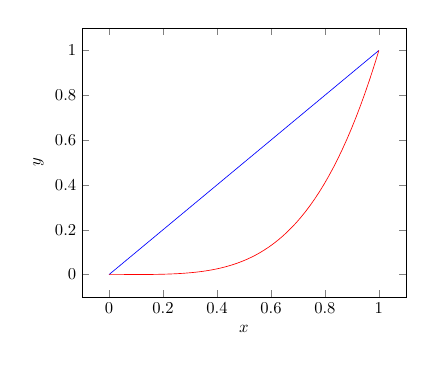
\begin{tikzpicture}[scale=0.6]
      \begin{axis}[
        xlabel=$x$,
        ylabel={$y$}
      ]
        \addplot+[mark=none,domain=0:1,samples=60]{x};
        \addplot+[mark=none,domain=0:1,samples=60]{x^4};
      \end{axis}
    \end{tikzpicture}
\end{figure}

\begin{align*}
    \int_{0}^{1} \int_{x^4}^{x} (x-1) \hspace{2pt} \mathrm{d}y \hspace{1pt} \mathrm{d}x &=
        \int_{0}^{1} \int_{y}^{y^{\nicefrac{1}{4}}} (x-1) \hspace{2pt} \mathrm{d}x \hspace{1pt} \mathrm{d}y\\
    &= \int_0^1 \left. \frac{x^2}{2}-x \right|_y^{y^{\nicefrac{1}{4}}} \mathrm{d}y\\
    &= \int_0^1 \left[  \frac{y^{\nicefrac{1}{2}}}{2} - y^{\nicefrac{1}{4}}   \right] - \left[\frac{y^2}{2} - y\right] \mathrm{d}y\\
    &= \left. \frac{y^{\nicefrac{3}{2}}}{3} - \frac{4y^{\nicefrac{5}{4}}}{5} - \frac{y^3}{6} + \frac{y^2}{2} \right|_0^1\\
    &= \frac{1}{3} - \frac{4}{5} - \frac{1}{6} +\frac{1}{2}\\
    &= -\frac{2}{15}
\end{align*}

\chapter{Lecture 15}
\label{chap:Lecture 15}

\section{Section 14.4}
\label{sec:Section 14.4}

\subsection{Problem 2}
\label{sub:Problem 2}
\begin{align*}
    \int_{0}^{2\pi} \int_{0}^{3\sin\theta} r \hspace{2pt} \mathrm{d}r \hspace{1pt} \mathrm{d}\theta &=
        \int_0^{2\pi} \left. \frac{r^2}{2} \right|_0^{3\sin\theta} \mathrm{d} \theta \\
    &= \int_0^{2\pi} \frac{9\sin^2\theta}{2} \mathrm{d} \theta \\
    &= \frac{9}{2}\int_0^{2\pi} \frac{1-\cos{2 \theta }}{2}\mathrm{d} \theta \\
    &= \frac{9}{4}\left[ 2\pi - \left. \frac{\sin\phi}{2}\right|_0^{4\pi}\right]\\
    &= \frac{9\pi}{2}
\end{align*}

\subsection{Problem 6}
\label{sub:Problem 6}
Assuming the problem meant to ask for area inside $r=2$ and outside $r = 2\cos\theta$, as $r = 2\cos\theta$ lies entierly within $r=2$.
\begin{align*}
    A = A_{outer}-A_{inner} &= \int_{0}^{2\pi} \int_{0}^{2} r           \hspace{2pt} \mathrm{d}r \hspace{1pt} \mathrm{d}\theta -
                               \int_{0}^{\pi} \int_{0}^{3\cos\theta} r \hspace{2pt} \mathrm{d}r \hspace{1pt} \mathrm{d}\theta \\
                            &= \int_{0}^{2\pi}  2           \hspace{2pt} \mathrm{d}\theta -
                               \int_{0}^{\pi} \frac{4\cos^2\theta}{2} \hspace{1pt} \mathrm{d}\theta \\
                            &= 4\pi - 2\int_0^{\pi} \cos^2\theta \hspace{1pt} \mathrm{d}\theta \\
                            &= 4\pi - \pi \\
                            &= 3\pi \\
\end{align*}
Care must be taken to not simply integrate $\int_{0}^{2\pi} \int_{2\cos\theta}^{2} r\hspace{2pt} \mathrm{d}r \hspace{1pt} \mathrm{d}\theta$, as this double counts the area of the interiaor cricle, which is of period $\pi$, rather than $2\pi$.

\subsection{Problem 16}
\label{sub:Problem 16}
\begin{align*}
    \int_0^1 \int_x^1 x^2 \hspace{2pt} \mathrm{d}y \hspace{1pt} \mathrm{d}x
        &= \left.\int_0^1 x^2y\right|_x^1  \hspace{2pt} \mathrm{d}x\\
        &= \int_0^1 x^2-x^3 \hspace{2pt} \mathrm{d}x\\
        &= \left.\frac{x^3}{3}-\frac{x^4}{4}\right|_0^1\\
        &= \nicefrac{1}{12}
\end{align*}
This doesn't fulfill the requirement of first substituting to polar coordiantes. But whatever.

\subsection{Problem 22}
\label{sub:Problem 22}
\begin{align*}
    \int_0^{2\pi} \int_0^{1+\cos\theta} 1 + x \hspace{2pt} \mathrm{d}r \hspace{1pt} \mathrm{d} \theta
        &= \int_0^{2\pi} \int_0^{1+\cos\theta} 1 + r\cos\theta \hspace{2pt} \mathrm{d}r \hspace{1pt} \mathrm{d} \theta \\
        &= \int_0^{2\pi}  1 + \cos\theta + \left. \frac{r^2 \cos\theta}{2}\right|_0^{1+\cos\theta} \hspace{2pt} \mathrm{d} \theta \\
        &= \int_0^{2\pi}  1 + \cos\theta + \frac{\left[1+2\cos\theta + \cos^2\theta\right]\cos\theta}{2} \hspace{2pt} \mathrm{d} \theta \\
        &= \int_0^{2\pi}  1 + \frac{2\cos^2\theta}{2} \hspace{2pt} \mathrm{d} \theta \\
        &= 3\pi
\end{align*}
It is convienent to make use of the fact that $\sin$ and $\cos$ will always have an integral of 0 when their operand iterates over an integral number of periods.

\subsection{Problem 24}
\label{sub:Problem 24}
We must first determine an appropriate bounding surface:
\begin{align*}
    &z_{hi}=12-2x^2-y^2&&&z_{lo}=x^2+2y^2&\\
    &&z_{hi} &= z_{lo}&& \\
    &&12-2x^2-y^2&=x^2+2y^2&&\\
    &&4 &= x^2 + y^2&&\\
\end{align*}
The enclosed volume is thus bounded by $x^2 + y^2 \leq 4$ on the $x-y$ plane, thus: $r \leq 2$
\begin{align*}
    \int_0^{2\pi} \int_0^{2} \left[\left(12-2x^2-y^2\right)-\left(x^2+2y^2\right)\right]r\hspace{2pt} \mathrm{d}r \hspace{1pt} \mathrm{d} \theta
        &= \int_0^{2\pi} \int_0^{2} \left[12-3x^2-3y^2\right]r\hspace{2pt} \mathrm{d}r \hspace{1pt} \mathrm{d} \theta \\
        &= \int_0^{2\pi} \int_0^{2} \left[12-3\left(x^2+y^2\right)\right]r\hspace{2pt} \mathrm{d}r \hspace{1pt} \mathrm{d} \theta \\
        &= \int_0^{2\pi} \int_0^{2} \left[12-3\left(r^2\cos^2\theta+r^2\sin^2\theta\right)\right]r\hspace{2pt} \mathrm{d}r \hspace{1pt} \mathrm{d} \theta \\
        &= \int_0^{2\pi} \int_0^{2} \left[12-3r^2\right]r\hspace{2pt} \mathrm{d}r \hspace{1pt} \mathrm{d} \theta \\
        &= \int_0^{2\pi} \int_0^{2} 12r-3r^3\hspace{2pt} \mathrm{d}r \hspace{1pt} \mathrm{d} \theta \\
        &= \int_0^{2\pi} \left. 6r^2-\frac{3r^4}{4}\right|_0^2 \hspace{2pt} \mathrm{d} \theta \\
        &= \int_0^{2\pi} 12 \hspace{2pt} \mathrm{d} \theta  \\
        &= 24\pi
\end{align*}

\subsection{Problem 30}
\label{sub:Problem 30}
\begin{align*}
    \int_0^{\pi} \int_0^{2a\sin\theta} r^2 \cdot r \hspace{2pt} \mathrm{d}r \hspace{1pt} \mathrm{d} \theta
    &= \int_0^{\pi} \int_0^{2a\sin\theta} r^3 \hspace{2pt} \mathrm{d}r \hspace{1pt} \mathrm{d} \theta  \\
    &= \int_0^{\pi} \left. \frac{r^4}{4} \right|_0^{2a\sin^4\theta}\hspace{2pt} \mathrm{d} \theta  \\
    &= \int_0^{\pi} \frac{16a^4\sin^4 \theta}{4} \hspace{2pt} \mathrm{d} \theta \\
    &= 4a^4\int_0^{\pi} \sin^4 \theta \hspace{2pt} \mathrm{d} \theta \\
    &= \frac{a^4}{2}\int_0^{\pi} 3 - 4\cos 2\theta + \cos 4\theta \hspace{2pt} \mathrm{d} \theta \\
    &= \frac{a^4}{2}\int_0^{\pi} 3  \hspace{2pt} \mathrm{d} \theta \\
    &= \frac{3\pi a^4}{2}
\end{align*}
It is once more convienent to make use of the fact that $\sin$ and $\cos$ will always have an integral of 0 when their operand iterates over an integral number of periods.


\section{Section 14.5}
\label{sec:Section 14.5}

\subsection{Problem 2}
\label{sub:Problem 2}
\begin{align*}
    &&m &= \int_2^4 \int_1^3 1 \hspace{2pt} \mathrm{d}x \hspace{1pt} \mathrm{d}y = 4&&\\
    \bar x &= \frac{1}{m} \int_2^4 \int_1^3 x \hspace{2pt} \mathrm{d}x \hspace{1pt} \mathrm{d}y &&& \bar y &= \frac{1}{m} \int_2^4 \int_1^3 y \hspace{2pt} \mathrm{d}x \hspace{1pt} \mathrm{d}y\\
    \bar x &= \frac{1}{4} \int_2^4 \left. \frac{x^2}{2}\right|_1^3 \hspace{2pt} \mathrm{d}y &&& \bar y &= \frac{1}{4} \int_2^4 2y \hspace{2pt} \mathrm{d}y\\
    \bar x &= \frac{1}{4} \int_2^4 4 \hspace{2pt} \mathrm{d}y &&& \bar y &= \left. \frac{1}{4} y^2\right|_2^4 \hspace{2pt} \mathrm{d}y\\
    \bar x &= 2 &&& \bar y &= 3\\
    && \left(\bar x, \bar y\right) &= (2,3) &&
\end{align*}

\subsection{Problem 6}
\label{sub:Problem 6}
The problem is made simpler by invoking the argument of symmetry, and only evaluating the y centroid of one half of the reigion, knowing that the x centriod will be at the point of symmetry: $\bar{x} = 1$.
\begin{align*}
    m &= \int_0^2 \int_y^1 1  \hspace{2pt} \mathrm{d}x \hspace{1pt} \mathrm{d}y\\
    &= \int_0^1 1-y  \hspace{2pt} \mathrm{d}y\\
    &= \nicefrac{1}{2}\\
\end{align*}
\begin{align*}
    \bar{y} &= \frac{1}{m} \int_0^2 \int_y^1 y  \hspace{2pt} \mathrm{d}x \hspace{1pt} \mathrm{d}y\\
    &= 2 \int_0^2 y(1-y)  \hspace{2pt} \mathrm{d}y\\
    &= 2 \int_0^2 y-y^2  \hspace{2pt} \mathrm{d}y\\
    &= 2 \left. \frac{y^2}{2}-\frac{y^3}{3} \right|_0^1\\
    &= \nicefrac{1}{3}\\
    \left(\bar x, \bar y\right) &= (1,\nicefrac{1}{3})
\end{align*}

\subsection{Problem 14}
\label{sub:Problem 14}
The problem is made simpler by invoking the argument of symmetry, and only evaluating the x centroid of one half of the reigion, knowing that the y centriod will be at the point of symmetry: $\bar{y} = 0$.
\begin{align*}
    m &= \int_0^9 \int_{-\sqrt{9-x}}^{\sqrt{9-x}} x^2  \hspace{2pt} \mathrm{d}y \hspace{1pt} \mathrm{d}x\\
    &= -2 \int_9^0 (9-u)^2 \sqrt{u}  \hspace{2pt} \mathrm{d}u\\
    &= -2 \int_9^0 81u^{\nicefrac{1}{2}} - 18 u^{\nicefrac{3}{2}} + u^{\nicefrac{5}{2}} \hspace{2pt} \mathrm{d}u\\
    &= \frac{23328}{35}\\
\end{align*}
\begin{align*}
    \bar{x} &= \frac{1}{m}\int_0^9 \int_{-\sqrt{9-x}}^{\sqrt{9-x}} x^3  \hspace{2pt} \mathrm{d}y \hspace{1pt} \mathrm{d}x\\
    &= -2 \frac{35}{23328} \int_9^0 (9-u)^3 \sqrt{u}  \hspace{2pt} \mathrm{d}u\\
    &= -2 \frac{35}{23328} \int_9^0 729u^{\nicefrac{1}{2}} - 243 u^{\nicefrac{3}{2}} + 27u^{\nicefrac{5}{2}} - u^{\nicefrac{7}{2}} \hspace{2pt} \mathrm{d}u\\
    &= 6\\
    \left(\bar x, \bar y\right) &= (6,0)
\end{align*}


\subsection{Problem 24}
\label{sub:Problem 24}
\begin{align*}
    m &= \int_{-1}^3 \int_{x^2}^{2x+3} x^2  \hspace{2pt} \mathrm{d}y \hspace{1pt} \mathrm{d}x\\
    &=   \int_{-1}^3 \left[2x+3-x^2\right] x^2  \hspace{2pt} \mathrm{d}x\\
    &= \frac{96}{5}\\
\end{align*}
\begin{align*}
    \bar{x} &= \frac{1}{m} \int_{-1}^3 \int_{x^2}^{2x+3} x^3  \hspace{2pt} \mathrm{d}y \hspace{1pt} \mathrm{d}x &
    \bar{y} &= \frac{1}{m} \int_{-1}^3 \int_{x^2}^{2x+3} x^2 y  \hspace{2pt} \mathrm{d}y \hspace{1pt} \mathrm{d}x\\
    &= \frac{5}{96} \int_{-1}^3 \left[2x+3-x^2\right] x^3  \hspace{2pt} \mathrm{d}x&
    &= \frac{5}{96} \int_{-1}^3 \left[2x+3-x^2\right] x^3  \hspace{2pt} \mathrm{d}x\\
    &= \frac{17}{9}&
    &= \frac{5}{2\cdot96} \int_{-1}^3 \left[(2x+3)^2-(x^2)^2\right] x^2  \hspace{2pt} \mathrm{d}x\\
    &&&= \frac{379}{168}\\
\end{align*}
Thus $\left(\bar x, \bar y\right) = (\frac{17}{9},\frac{379}{168})$, or approximately $(1.89,2.26)$.



\begingroup
\let\cleardoublepage\clearpage
\part{Online}
\endgroup

\chapter{Problem 1}
\label{chap:Problem 1}
We start by simpifying the problem to the maximum volume of a right cuboid with a diagonal
between the origin and a point on the unit sphere in the first octant. We then attempt to maximize
the volume, $f(x,y,z) = xyz$, under the condition $x^2+y^2+z^2 = 1$, or $g(x,y,z) = x^2+y^2+z^2 -1 =0$,
using Lagrange Multipliers:
$$L(x,y,z,\lambda) = xyz - \lambda \left(x^2+y^2+z^2-1\right)$$

Setting $x, y, z$ partials to 0 yields:
\begin{align*}
    \pder{L}{x} &= 1 - 2x\lambda = 0 & \pder{L}{y} &= 1 - 2y\lambda = 0 & \pder{L}{z} &= 1 - 2z\lambda = 0\\
    &&x = y = z &= \frac{1}{2\lambda}&&
\end{align*}
Setting $\lambda$ partial to 0 yields:
\begin{align*}
    \pder{L}{\lambda} &= x^2 + y^2 + z^2 -1 = 0\\
    3\left(\frac{1}{2\lambda}\right)^2 &= 1\\
    \lambda &= \frac{\sqrt{3}}{2}\\
    x = y = z = \frac{1}{2\lambda} &= \frac{1}{\sqrt{3}}
\end{align*}

Volume is maximized when $x = y =z = \frac{1}{\sqrt{3}}$, when the box is a cube, with volume $8\left(\frac{1}{\sqrt{3}}\right)^3 = \frac{8}{3\sqrt{3}}$

\chapter{Problem 2}
\label{chap:Problem 1}
Function: $$f(x,y) = x^2-2xy+7y^2$$
Condition: $$x^2 + 4y^2 =1 \Longrightarrow g(x,y) = x^2 + 4y^2 -1 = 0$$
In Lagrange equation:
\begin{align*}
    L(x,y,\lambda) &= f(x,y) - \lambda g(x,y)\\
    &= x^2-2xy+7y^2 - \lambda \left(x^2 + 4y^2 -1\right)
\end{align*}
Setting partials to 0:
\begin{align*}
    \pder{L}{x} &= 2x - 2y - 2\lambda x = 0 &&& \pder{L}{y} &= 14y - 2x - 8\lambda y = 0\\
    x &= \frac{y}{1-\lambda}&&  & y &= \frac{x}{7-4\lambda}\\
    &&x &= \frac{\frac{x}{7-4\lambda}}{1-\lambda}&&\\
    && \left(7-4\lambda\right)\left(1-\lambda\right) &= 1&&\\
    &&  6 - 11\lambda + 4\lambda^2&= 0 && \\
    && \lambda &= \left[ \nicefrac{3}{4}, 2\right]\\
    \lambda & = 2 &&& \lambda &= \nicefrac{3}{4}\\
    x & = \frac{y}{1-2} &&& y &= \frac{x}{7-3}\\
    x &= -y &&& x &= 4y\\
    5y^2 - 1 &= 0 &&& 20y^2 &= 1\\
    y = -x &= \pm\sqrt{\nicefrac{1}{5}} &&& y &= \pm\sqrt{\nicefrac{1}{20}}\\
    &&&& x = 4y &= \pm\sqrt{\nicefrac{16}{20}}
\end{align*}
Plugging back into original equation, maximums are at $f(\sqrt{\nicefrac{1}{5}}, -\sqrt{\nicefrac{1}{5}})$ and $f(-\sqrt{\nicefrac{1}{5}}, \sqrt{\nicefrac{1}{5}})$, where $f(x,y) = 2$, and minumums are at $f(\sqrt{\nicefrac{16}{20}}, \sqrt{\nicefrac{1}{20}})$ and $f(-\sqrt{\nicefrac{16}{20}}, - \sqrt{\nicefrac{1}{20}})$,  where $f(x,y) = \nicefrac{3}{4}$.




\chapter{Problem 3}
\label{chap:Problem 1}
\begin{align*}
    r &= \sqrt{x^2 + y^2} & \theta &= \tan^-1 \frac{y}{x}\\
    \pder{r}{x} &= \frac{x}{\sqrt{x^2+y^2}} & \pder{\theta}{x} &= \frac{-y}{y^2+x^2}\\
    \pder{r}{y} &= \frac{y}{\sqrt{x^2+y^2}} & \pder{\theta}{y} &= \frac{x}{y^2+x^2}\\
\end{align*}
\begin{align*}
    \left|\nabla f\right| ^2 &= \pder{f}{x}^2 + \pder{f}{y}^2\\
    &= \left(\pder{f}{r} \pder{r}{x} + \pder{f}{\theta} \pder{\theta}{x}\right)^2 +
       \left(\pder{f}{r} \pder{r}{y} + \pder{f}{\theta} \pder{\theta}{y}\right)^2\\
    &= \left(\pder{f}{r} \frac{x}{\sqrt{x^2+y^2}} - \pder{f}{\theta} \frac{y}{y^2+x^2}\right)^2 +
       \left(\pder{f}{r} \frac{y}{\sqrt{x^2+y^2}} + \pder{f}{\theta} \frac{x}{y^2+x^2}\right)^2\\
\end{align*}
\begin{align*}
    x &= r\cos\theta& & & y&= r\sin\theta\\
    &&x^2 + y^2 &= r^2 \left(\cos^2 \theta + \sin^2\theta\right)\\
    &&&= r^2
\end{align*}
\begin{align*}
    \left|\nabla f\right| ^2
    &= \left(\pder{f}{r} \frac{x}{\sqrt{r^2}} - \pder{f}{\theta} \frac{y}{r^2}\right)^2 +
       \left(\pder{f}{r} \frac{y}{\sqrt{r^2}} + \pder{f}{\theta} \frac{x}{r^2}\right)^2\\
    &= \left(\pder{f}{r} \frac{r\cos\theta}{r} - \pder{f}{\theta} \frac{r\sin\theta}{r^2}\right)^2 +
       \left(\pder{f}{r} \frac{r\sin\theta}{r} + \pder{f}{\theta} \frac{r\cos\theta}{r^2}\right)^2\\
    &= \left(\pder{f}{r} \cos\theta - \pder{f}{\theta} \frac{\sin\theta}{r}\right)^2 +
       \left(\pder{f}{r} \sin\theta + \pder{f}{\theta} \frac{\cos\theta}{r}\right)^2\\
\end{align*}

\chapter{Problem 4}
\label{chap:Problem 1}
\begin{align*}
    \frac{dF}{dt} &= \pder{F}{x} \der{x}{t} + \pder{F}{y} \der{y}{t} + \pder{F}{z} \der{z}{t}\\
    &= -2xF_0e^{-\left(x^2 + y^2 +z^2\right)} * \peren{-1} + -2yF_0e^{-\left(x^2 + y^2 +z^2\right)} * \peren{0} + -2zF_0e^{-\left(x^2 + y^2 +z^2\right)} * \peren{-2\peren{1-t}}\\
    &= -2xF_0e^{-\left(x^2 + y^2 +z^2\right)} * \peren{-1} + -2zF_0e^{-\left(x^2 + y^2 +z^2\right)} * \peren{-2\peren{1-t}}\\
    &= F_0e^{-\left(\peren{1-t}^2 + \peren{\peren{1-t}^2}^2\right)}
        \peren{2\peren{1-t} + 2\peren{1-t}^2\peren{2\peren{1-t}}}\\
    &= F_0e^{-\left(\peren{1-t}^2 + \peren{\peren{1-t}^2}^2\right)}
        \peren{2\peren{1-t} + 4\peren{1-t}^3}\\
\end{align*}

\chapter{Problem 5}
\label{chap:Problem 1}
Assume base starts at origin and has diagonal going from $\peren{0,0}$ to $\peren{j,k}$. Through adjusting $a,b,c,d,j,$ and $k$, this model can be shown to represent any possible rectangular prism with varying side lengths.
\begin{align*}
    V &= \int_0^j \int_0^k ax + by +c \hspace{2pt} \mathrm{d}y \hspace{1pt} \mathrm{d}x\\
    &= \int_0^j \peren{k-0} \peren{ax + c} + \frac{bk^2}{2} \hspace{2pt} \mathrm{d}x\\
    &= kcj+ \frac{jbk^2}{2} \int_0^j kax \hspace{2pt} \mathrm{d}x\\
    &= kcj+ \frac{jbk^2}{2} + \frac{kaj^2}{2} \\
    &= kj \peren{\frac{aj}{2} + \frac{bk}{2} + c}\\
\end{align*}
\begin{align*}
    l_0 &= z(0,0) = a(0) + b(0) + c = c\\
    l_1 &= z(j,0) = a(j) + b(0) + c = aj + c\\
    l_2 &= z(0,k) = a(0) + b(k) + c = bk + c\\
    l_3 &= z(j,j) = a(j) + b(k) + c = aj + bk + c\\
    l_{avg} &= \frac{1}{4} \sum l_i\\ &= \frac{4c + 2aj + 2bk}{4} \\&= c + \frac{aj}{2} + \frac{bk}{2}\\
\end{align*}
\begin{align*}
    A_{base} &= kj\\
    A_{base} \cdot l_{avg} &= kj \cdot \peren{c + \frac{aj}{2} + \frac{bk}{2}} = \int_0^j \int_0^k ax + by +c \hspace{2pt} \mathrm{d}y \hspace{1pt} \mathrm{d}x\\
\end{align*}
$$\text{Which Was What We Wanted}$$

\chapter{Problem 6}
\label{chap:Problem 1}
\begin{figure}[!h]
\centering
    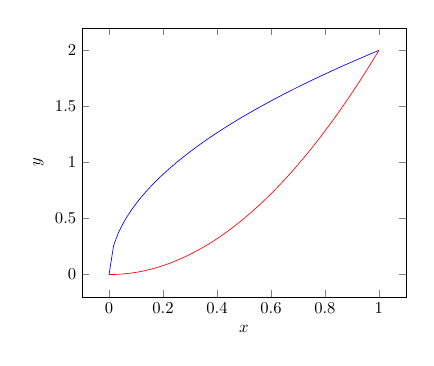
\begin{tikzpicture}[scale=0.6]
      \begin{axis}[
        xlabel=$x$,
        ylabel={$y$}
      ]
        \addplot+[mark=none,domain=0:1,samples=60]{sqrt(4*x)};
        \addplot+[mark=none,domain=0:1,samples=60]{2*x^2};
      \end{axis}
    \end{tikzpicture}

    Plot for $y^2 = 4ax$ and $x^2 = \nicefrac{ay}{2}$ when $a=1$.
\end{figure}




\begin{align*}
    y^2 &= 4ax \Longrightarrow y=\sqrt{4ax} \text{ or, equivalently } x = \frac{y^2}{4a}\\
    x^2 &= \frac{ay}{2} \Longrightarrow x=\sqrt{\frac{ay}{2}} \text{ or, equivalently } y = \frac{2x^2}{a}\\
\end{align*}
\begin{align*}
    A &= \int_0^{2a} \sqrt{\frac{ay}{2}} - \frac{y^2}{4a} \hspace{2pt} \mathrm{d}y &
     A &= \int_0^{a} \sqrt{4ax} - \frac{2x^2}{a} \hspace{2pt} \mathrm{d}x\\
    &= \sqrt{\frac{a}{2}} \int_0^{2a} \sqrt{y}\hspace{2pt} \mathrm{d}y - \frac{1}{4a} \int_0^{2a} y^2 \hspace{2pt} \mathrm{d}y &
     &= 2\sqrt{a} \int_0^{a} \sqrt{x} \hspace{2pt} \mathrm{d}x- \frac{2}{a} \int_0^{a} x^2 \hspace{2pt} \mathrm{d}x\\
    &= \sqrt{\frac{a}{2}} \left[\frac{2y^{\nicefrac{3}{2}}}{3}\right]_0^{2a}-
            \frac{1}{4a}  \left[\frac{y^3}{3}\right]_0^{2a} &
     &= 2\left[\frac{2}{3} x \sqrt{ax}\right]_0^a -
            \frac{2}{a} \left[\frac{y^3}{3}\right]_0^{a}\\
     &= \sqrt{\frac{a}{2}}\frac{4a\sqrt{2a}}{3} - \frac{2a^2}{3} & &= \frac{4a^2}{3} - \frac{2a^2}{3}\\
     &= \frac{2a^2}{3} & &= \frac{2a^2}{3}\\
\end{align*}



\chapter{Problem 7}
\label{chap:Problem 1}
\begin{align*}
    I^2 = \int_0^\infty \negmedspace e^{-x^2} \hspace{2pt} \mathrm{d} x
        \int_0^\infty \negmedspace e^{-y^2} \hspace{2pt} \mathrm{d} y
        &= \int_0^\infty \negthickspace \int_0^\infty \negmedspace e^{-\peren{x^2+y^2}} \hspace{2pt} \mathrm{d} x \hspace{1pt} \mathrm{d} y\\
        &= \int_0^{\nicefrac{\pi}{2}} \negthickspace \int_0^\infty \negmedspace e^{-r^2}r \hspace{2pt} \mathrm{d} r \hspace{1pt} \mathrm{d} \theta\\
        &= -\frac{1}{2} \int_0^{\nicefrac{\pi}{2}} \negthickspace \int_0^{-\infty} \negmedspace e^{u} \hspace{2pt} \mathrm{d} u \hspace{1pt} \mathrm{d} \theta\\
        &= -\frac{1}{2} \int_0^{\nicefrac{\pi}{2}} \negmedspace e^{-\infty} - e^{0} \hspace{2pt} \mathrm{d} \theta\\
        &= -\frac{1}{2} \int_0^{\nicefrac{\pi}{2}} \negmedspace -1 \hspace{2pt} \mathrm{d} \theta\\
        I^2 &= \nicefrac{\pi}{4}\\
        I = \int_0^\infty \negmedspace e^{-x^2} \hspace{2pt} \mathrm{d} x &= \frac{\sqrt{\pi}}{2}\\
\end{align*}


\chapter{Problem 8}
\label{chap:Problem 1}


\begin{figure}[!h]
\centering
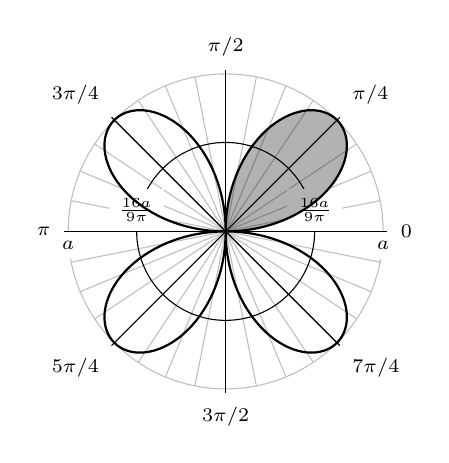
\begin{tikzpicture}[>=latex,scale=0.5]

% Draw the lines at multiples of pi/12
\foreach \ang in {0,...,31} {
  \draw [lightgray] (0,0) -- (\ang * 180 / 16:4);
}

% Concentric circles and radius labels

\draw [lightgray] (0,0) circle (4);
\draw (0,0) circle (2.26);

\node [fill=white] at (4, 0) [below] {\scriptsize $a$};
\node [fill=white] at (-4, 0) [below] {\scriptsize $a$};
\node [fill=white] at (2.26, 0) [above] {\scriptsize $\frac{16a}{9\pi}$};
\node [fill=white] at (-2.26, 0) [above] {\scriptsize $\frac{16a}{9\pi}$};

% Add the labels at multiples of pi/4
\foreach \ang/\lab/\dir in {
  0/0/right,
  1/{\pi/4}/{above right},
  2/{\pi/2}/above,
  3/{3\pi/4}/{above left},
  4/{\pi}/left,
  5/{5\pi/4}/{below left},
  7/{7\pi/4}/{below right},
  6/{3\pi/2}/below} {
  \draw (0,0) -- (\ang * 180 / 4:4.1);
  \node [fill=white] at (\ang * 180 / 4:4.2) [\dir] {\scriptsize $\lab$};
}

\fill [fill=black!50!black, opacity=0.3] plot [domain=0:pi/2] (xy polar cs:angle=\x r,radius= {4*sin(2*\x r)});
\draw [thick,color=black,domain=0:2*pi,samples=200,smooth] plot (xy polar cs:angle=\x r,radius= {4*sin(2*\x r)});

\end{tikzpicture}
\end{figure}

The area of entire curve will be that of shaded reigion, times 4. Average distance from origin of reigion will trivially be 0, as can be proven by invoking the argument of symmetry about $x=0$ and $y=0$. Perhaps the question is asking the average distance from origin for a single lobe? This can be shown to be $\frac{16a}{9\pi}$, and is marked on the above plot.
\begin{align*}
    A &= 4\int_0^{\nicefrac{\pi}{2}} \int_0^{a\sin{2\theta}} r \hspace{2pt} \mathrm{d} r \hspace{1pt} \mathrm{d} \theta &
        \bar{D} &= \frac{1}{\frac{A}{4}} \int_0^{\nicefrac{\pi}{2}} \int_0^{a\sin{2\theta}} r\sqrt{x^2 + y^2} \hspace{2pt} \mathrm{d} r \hspace{1pt} \mathrm{d} \theta \\
     &= 4\frac{1}{2} \left. \int_0^{\nicefrac{\pi}{2}} r^2\right|_0^{a\sin{2\theta}} \hspace{2pt} \mathrm{d}\theta&
         &= \frac{8}{a^2\pi} \int_0^{\nicefrac{\pi}{2}} \int_0^{a\sin{2\theta}} r\sqrt{r^2\peren{\cos^2 \theta + \sin^2 \theta}} \hspace{2pt} \mathrm{d} r \hspace{1pt} \mathrm{d} \theta \\
    &= 4\frac{a^2}{2} \int_0^{\nicefrac{\pi}{2}} \sin^2\peren{2\theta} \hspace{2pt} \mathrm{d}\theta&
         &= \frac{8}{a^2\pi} \int_0^{\nicefrac{\pi}{2}} \int_0^{a\sin{2\theta}} r^2 \hspace{2pt} \mathrm{d} r \hspace{1pt} \mathrm{d} \theta \\
    &= 4\frac{a^2}{2} \int_0^{\nicefrac{\pi}{2}} \frac{1-2\cos{4\theta}}{2} \hspace{2pt} \mathrm{d}\theta&
         &= \frac{8}{a^2\pi} \frac{a^3}{3} \int_0^{\nicefrac{\pi}{2}} \sin^3{2\theta} \hspace{2pt} \mathrm{d} \theta\\
    &= 4\frac{a^2}{4} \int_0^{\nicefrac{\pi}{2}} 1 \hspace{2pt} \mathrm{d}\theta -
      \frac{a^2}{2} \int_0^{\nicefrac{\pi}{2}} \negmadspace \peren{-2}\cos{4\theta} \hspace{2pt} \mathrm{d}\theta&
         &= \frac{4a}{3\pi} \int_0^{\nicefrac{\pi}{2}} 3\sin{\theta} - \sin{3\theta} \hspace{2pt} \mathrm{d} \theta\\
    &= 4\frac{a^2}{4} \int_0^{\nicefrac{\pi}{2}} 1 \hspace{2pt} \mathrm{d}\theta - 0&
     &= \frac{2a}{3\pi} \peren{3-\frac{1}{3}}\\
    A &= 4\frac{a^2\pi}{8} = \frac{a^2\pi}{2}  &    \bar{D} &= \frac{2a}{3\pi} \cdot \frac{8}{3} = \frac{16a}{9\pi}\\
\end{align*}





\end{document}
